\section{\textcolor{magenta}{Procédure de fermeture du lab}}


\begin{enumerate}
    \item Replacer le \textit{beam dump} devant la sortie du laser (voir figure~\ref{fig:beam-dump}).
    \item Sur le \textit{contrôleur du Verdi}, peser sur le bouton \textit{Shutter Open} (voir figure~\ref{fig:controleur-verdi}). On peut maintenant enlever les lunettes de sécurité.
    \item Sur l'interface d'accueil du logiciel \textit{Umoco}, cliquer sur X. Confirmer l'arrêt du logiciel \textit{Umoco}.
    \item Éteindre la caméra: mettre l'interrupteur \textit{Power} de \textit{On} à \textit{Off} (voir figure~\ref{fig:cam_power}).
\begin{center} $\ast\ast\ast$ Si vous avez d'autres échantillons à imager dans les prochains jours, passez tout de suite à l'étape~\ref{skip}. Puisque l'ouverture complète du laser peut être longue, on peut le laisser à \textit{On} quelques jours consécutifs. Il faut alors laisser la lumière rouge d'avertissement allumée.  $\ast\ast\ast$ \end{center}
    \item Tourner la clé de \textit{On} à \textit{Standby} sur le \textit{contrôleur du Verdi} (voir figure~\ref{fig:controleur-verdi}).
    \item Sur le \textit{contrôleur du Verdi}, aller dans \textit{LBO Settings} et mettre le \textit{'LBO'} sur l'état \textit{'Cooling'}. Peser deux fois sur \textit{Menu Exit}.
    \item Tourner la roulette pour atteindre une puissance de 0~W.
    \item \textcolor{magenta}{HELLO}
    \item Sur chaque refroidisseur (voir figure~\ref{fig:cooler}), peser sur le bouton \textit{Run/Standby}. Le message \textit{Standby Mode} devrait s'afficher.
    \item Derrière le \textit{contrôleur du Verdi}, mettre la bascule sur \textit{Off}.
    \item Sur le \textit{contrôleur du Mira} (voir figure~\ref{fig:controleurs}), mettre la bascule de gauche sur \textit{CW}.
    \item Éteindre la lumière rouge d'avertissement grâce à l'interrupteur \textcolor{magenta}{FIGURE}.
    \item \label{skip} Retirer la cuvette contenant l'échantillon.
    \item Retirer le liquide de la chambre à l'aide d'une pipette. Ce liquide est généralement réutilisable et peut être conservé dans un contenant à part.
    \item Rincer l'intérieur de la chambre à l'aide d'un flacon laveur d'eau (voir figure~\ref{fig:eau}).
    \item A l'aide d'une autre pipette, transvider les restants de liquides dans le bécher à déchets.
    \item Répéter les deux dernières étapes si nécessaire.
    \item Prendre un papier optique (voir figure~\ref{fig:papier}). Le plier jusqu'à grandeur voulue. Prendre soin de ne jamais toucher la partie du papier optique qui entrera en contact avec l'objectif. 
        \begin{figure}[H]
        \centering
        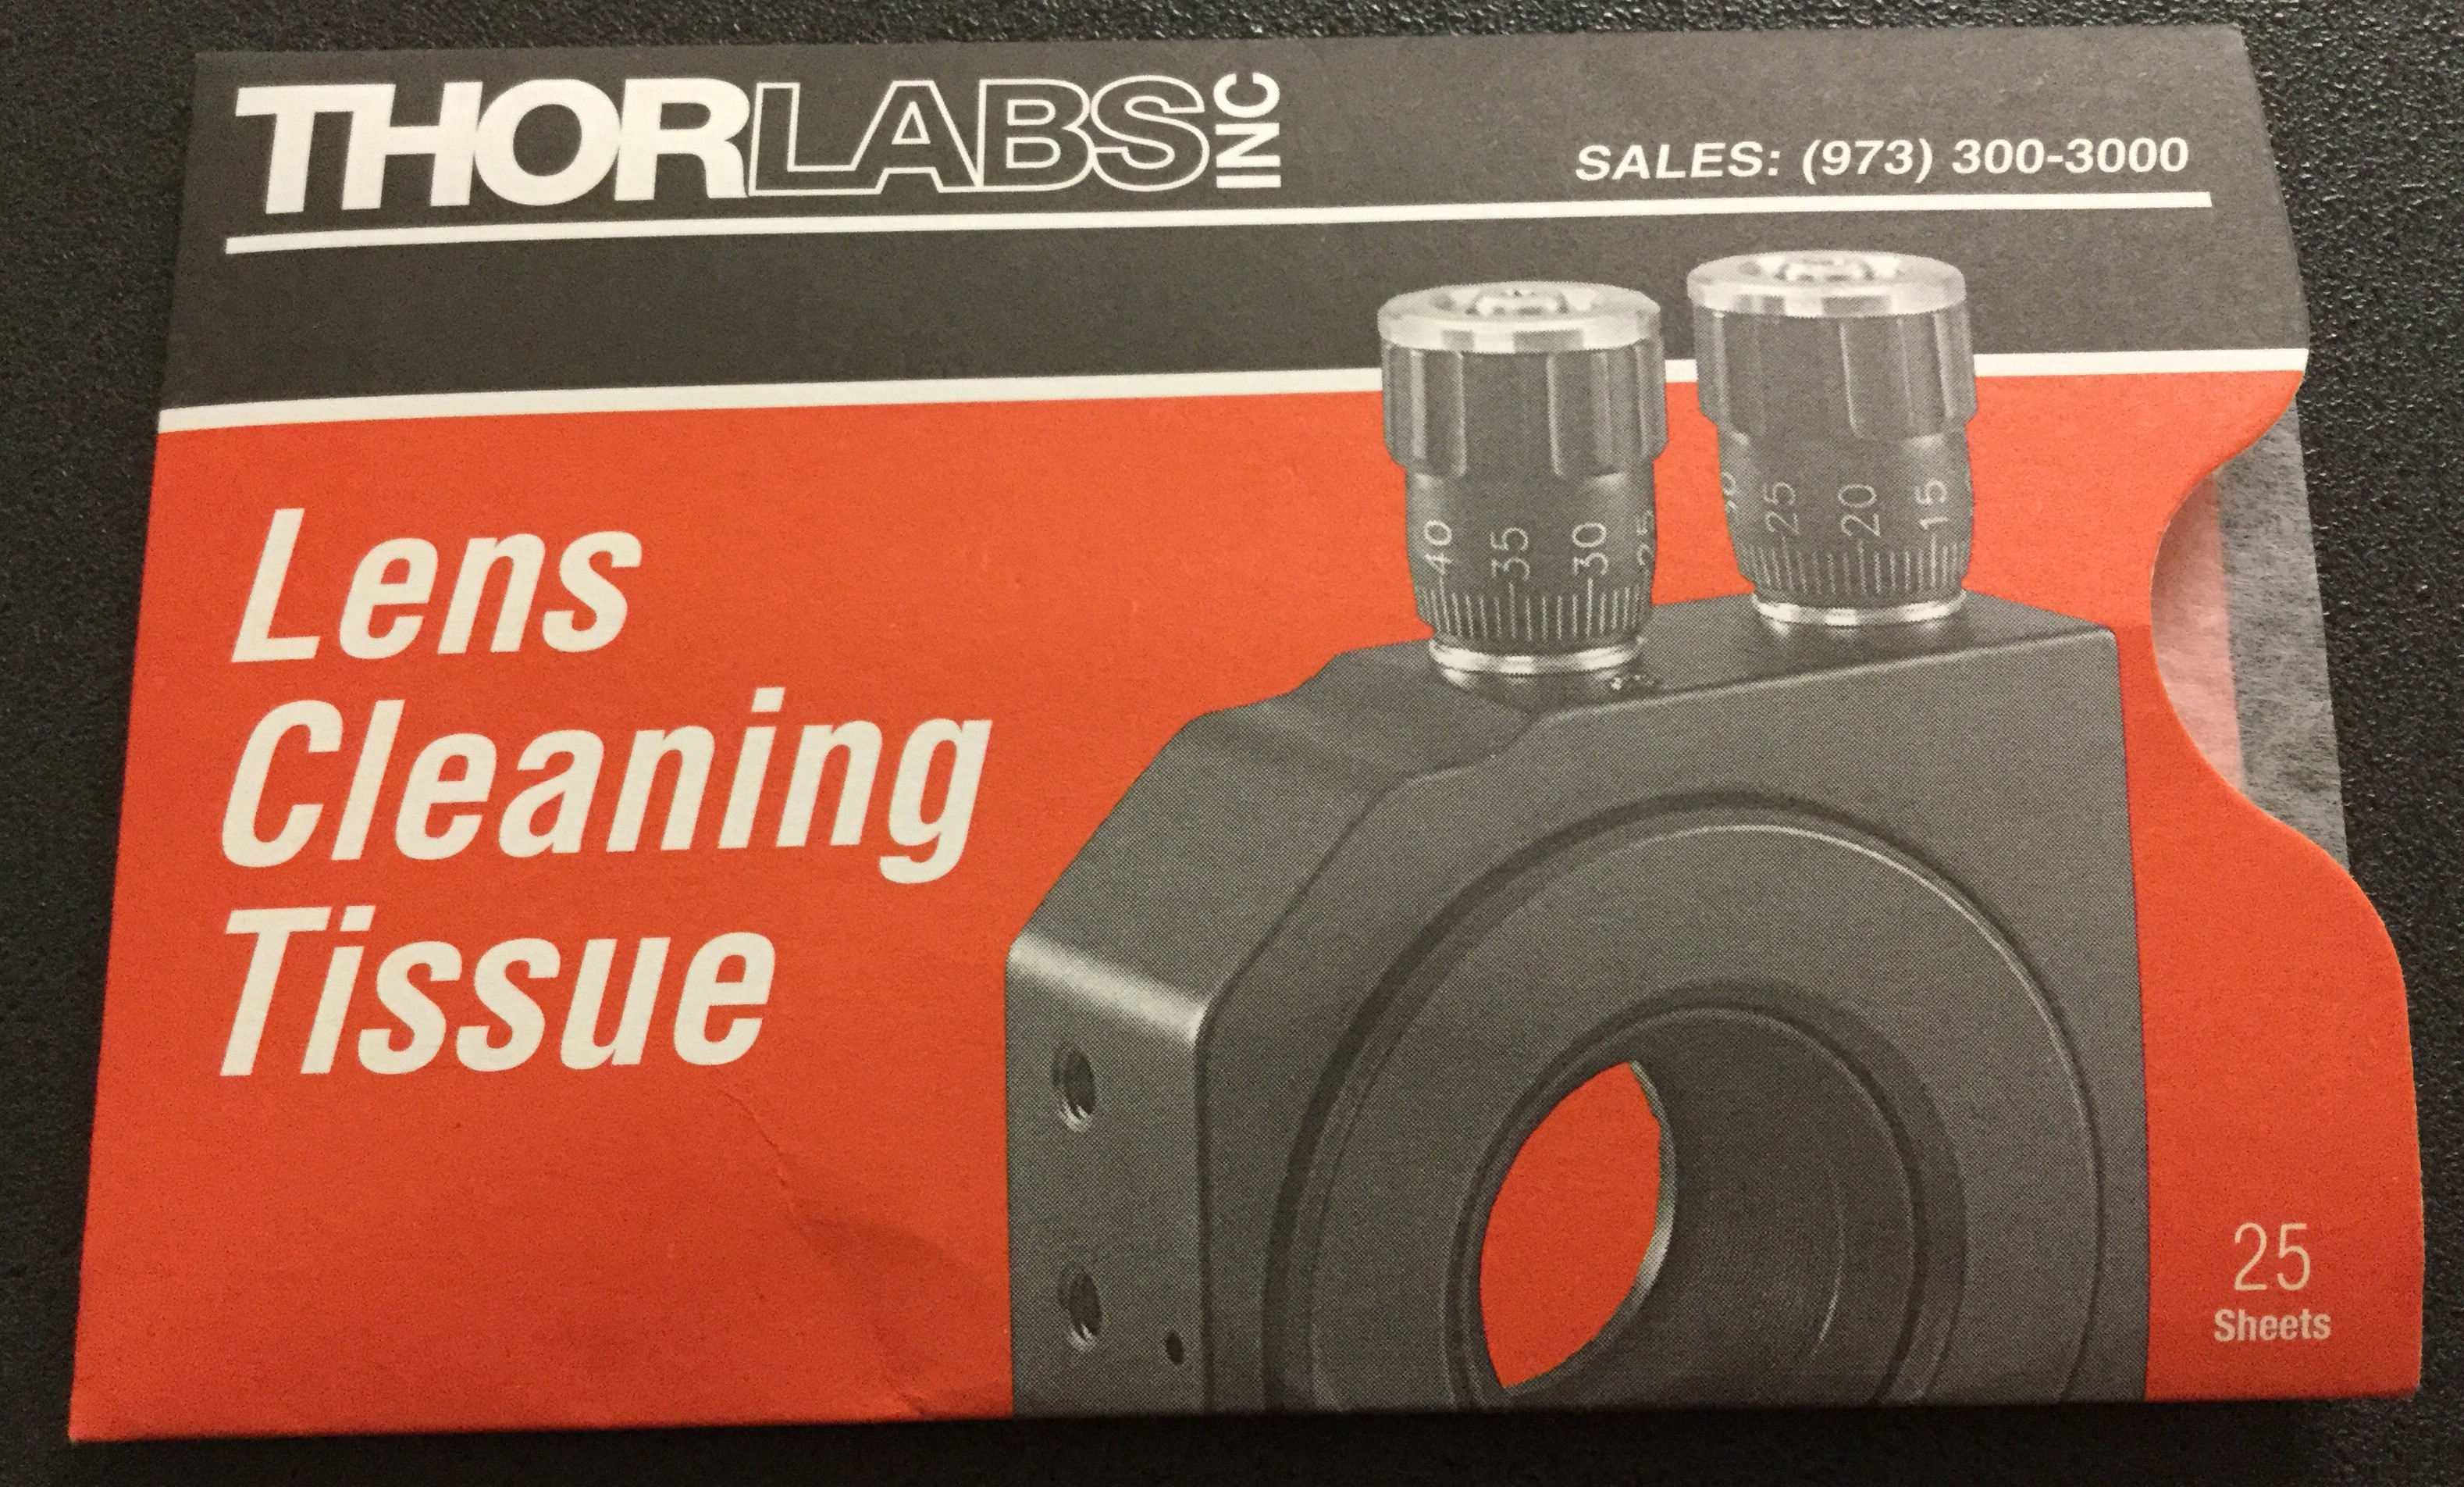
\includegraphics[width=5cm]{papier.jpg}
        \caption{Papier optique}
        \label{fig:papier}
        \end{figure}
    \item Passer doucement le papier sur l'objectif, et ce, une seule fois (pas d'aller-retour). Ne pas mettre de pression. Jeter le papier.
    \item Répéter les deux dernière étapes si nécessaire. Ne jamais utiliser deux fois le même papier optique.
    \item Au besoin, mettre des gants et utiliser un peu d'éthanol avec le papier optique.
    \item Remettre l'échantillon dans son contenant d'origine.
    \item Mettre des gants. Nettoyer la cuvette avec de l'éthanol. \item Si la cuvette est en verre: Laisser sécher à l'air libre. Ne pas essuyer.
\end{enumerate}